% !TEX root = ../main/main.tex
\section{Introduction}
Heat sinks are a commonly used heat exchangers with the purpose of transferring heat that are generated by electronic or mechanical devices \cite{wiki_hs}. In computers it is useful to be able to regulate the temperature of components like the central processing unit (CPU) or the graphic processing unit	(GPU). These units typically generate a lot of heat and it becomes necessary for optimal operation to dissipate this heat away to keep the temperature at an optimal level. This is typically done by using a heat sink together with a fan as seen in \textbf{Figure \ref{fig:heatsink_and_fan}}. 

\begin{wrapfigure}{r}{0.5\textwidth}
	\begin{center}
		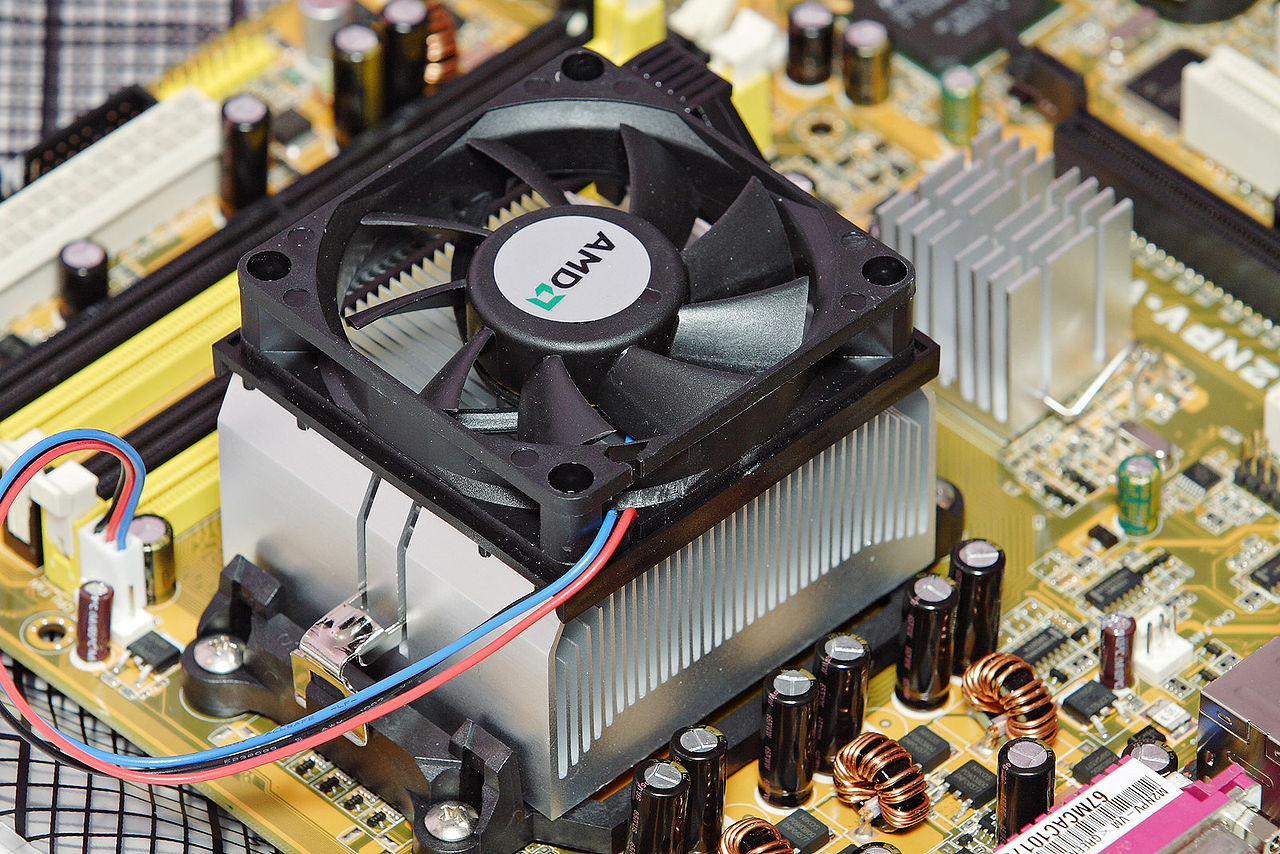
\includegraphics[width=0.48\textwidth]{../figures/heatsink_and_fan.jpg}
	\end{center}
	\caption{Heat sink and fan on processing unit. Source: \cite{wiki_hs}}
    \label{fig:heatsink_and_fan}
\end{wrapfigure}

When designing heat sinks one typically tries to maximize surface area in contact with the cooling medium surrounding it, such as air. There are several factors that affects the performance of a heat sink. In essence air velocity, choice of material, design and surface treatment are the most important ones. When choosing material one should look for good heat conductors which means that heat can be transferred though the material quickly. In many cases copper is used because of its excellent thermal efficiency.

In this project we will be trying to use a Finite Element Method to evaluate the effect of increasing the surface area on a simple heat sink design in two different ways. One ways is to extend the length of the fins, and the other is to increase the number of fins. We will keep the geometric properties of the heat sink base constant, meaning that we will only vary the geometry of the fins themselves. This report is divided into three main parts. In the \textit{Theory} part we will elaborate on the heat equation and show a finite element analysis which results in a linear system of equations. In the \textit{Numerical Implementations} part we will go through and explain the steps of implementing the numerical interpretation. In the \textit{Results and Discussion} we will present our results together with a discussion of their interpretation. Finally we will sum up our findings and suggest improvements in a conclusion. %TODO: Check the correct section names.